\documentclass[11pt,a4paper]{article}
\usepackage[utf8]{inputenc}
\usepackage[francais]{babel}
\usepackage[T1]{fontenc}
\usepackage{amsmath}
\usepackage{amsfonts}
\usepackage{graphicx}
\usepackage{amssymb}
\usepackage{fullpage}
\usepackage{fancybox}
\usepackage[Lenny]{fncychap}
\usepackage{gensymb}
\usepackage{color}
\usepackage{array}
\usepackage{url}
\usepackage{here}
\usepackage{ulem}
\usepackage[final]{pdfpages}
\usepackage{wrapfig}
\usepackage{subcaption}
\usepackage{listings}
\lstdefinestyle{Bash}
{language=bash,
keywordstyle=\color{blue},
backgroundcolor=\ttfamily\color{black},  
basicstyle=\color{green},
morekeywords={peter@kbpet},
alsoletter={:~$},
morekeywords=[2]{peter@kbpet:},
keywordstyle=[2]{\color{red}},
literate={\$}{{\textcolor{red}{\$}}}1 
         {:}{{\textcolor{red}{:}}}1
         {~}{{\textcolor{red}{\textasciitilde}}}1,
}
\newcommand{\code}[1]{\texttt{#1}}
\author{\textsc{De Mol} Maxime}
\title{Tuto compilation C sur Mac pour Eléments Finis}
\date{\today}

\begin{document}

\maketitle

\section{Introduction}

Salut à vous, tous les macoïdes qui galérez (ou allez galérer dans un futur proche) avec le problème 1 en éléments finis! Si tu es sur Windows, je vais te dire la même chose que nous a dis Olivier Bonaventure, "Tant pis pour toi"! Si tu es sur Linux, certains éléments vont être semblable, d'autre pas du tout, mais moi je m'en fout, je suis pas sur Linux. Et si enfin, tu es sur Mac, ce guide est pour toi!

\begin{figure}[H]

\includegraphics[width=\linewidth]{nouveau-logo-apple.jpg}
\end{figure}

\section{The easy way: Xcode}

Comme vous l'indique le titre de la section, il y a plusieurs façon de développer (= écrire des programmes barbants dans des langages bizarres) sur Mac. Personnellement j'en connais 2. La première, et la plus simple, consiste en l'utilisation de Xcode, ce programme développé par Apple, disponible seulement sur Mac, va vous assister énormément dans l'écriture de vos petites missions! Le modus operandi est très simple.

\subsection{Step 1 - Start}
\begin{minipage}[c]{.20\linewidth}

\includegraphics[width=\linewidth]{macapp.png}
\end{minipage} \hfill
\begin{minipage}[c]{.74\linewidth}
Direction le Mac App Store (si vous n'avez pas de Mac App Store sur votre Mac, c'est que probablement votre mac est trop vieux pour le dernier Xcode, donc passez directement à l'étape 2-bis).
\end{minipage}

\subsection{Step 2 - Get Xcode}
\begin{minipage}[c]{.40\linewidth}

\includegraphics[width=\linewidth]{getxcode.png}
\end{minipage} \hfill
\begin{minipage}[c]{.50\linewidth}
Simple. Cherchez pour "Xcode". Trouvez. Téléchargez. Done!
\end{minipage}

\subsection{Step 2 - bis}
\begin{minipage}[c]{.40\linewidth}
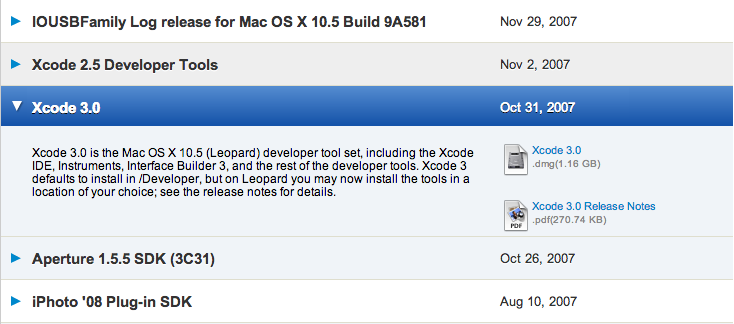
\includegraphics[width=\linewidth]{xcode3.png}
\end{minipage} \hfill
\begin{minipage}[c]{.50\linewidth}
Votre Mac est vieux, vous tournez sur Leopard, ou plus ancien? Il vous faut Xcode 3! Là, c'est plus compliqué que pour vos collègues plus moderne. Vous vous rendez ici: \url{https://developer.apple.com/downloads/index.action}. Vous devez créer un compte développeur, et une fois que vous avez accès à tous les ressources, naviguez vers la page 8, localisez Xcode 3, téléchargez, installez!
\end{minipage}

\subsection{Step 3 - New Project}
\begin{minipage}[c]{.40\linewidth}
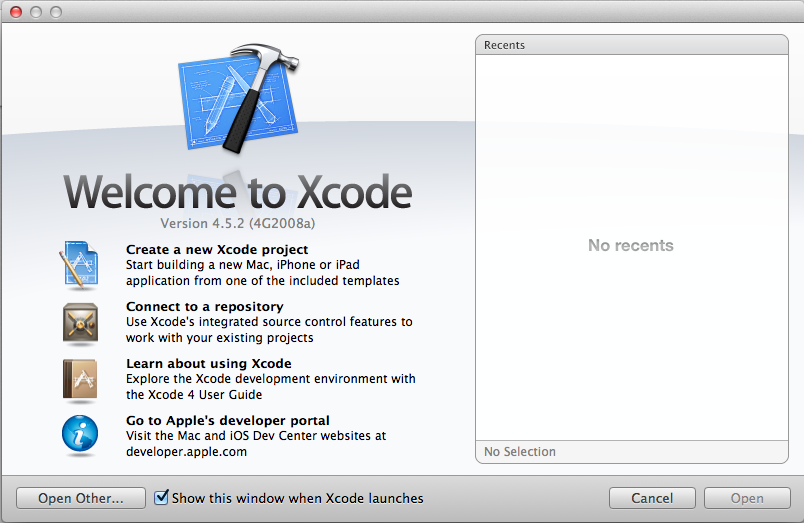
\includegraphics[width=\linewidth]{project.png}
\end{minipage} \hfill
\begin{minipage}[c]{.50\linewidth}
Vous devez créer un nouveau projet pour pouvoir commencer à travailler votre code! Pour cela, dans la page d'accueil de Xcode, vous choisissez "Create a new Xcode project" >> OSX >> Application >> Command Line Tool. Là vous donnez quelques détails, et choisissez bien dans Type : C. C'est important! Reste plus qu'à choisir la destination de votre dossier projet, and it's done!
\end{minipage}

\subsection{Step 4 - The Files}
\begin{minipage}[c]{.40\linewidth}
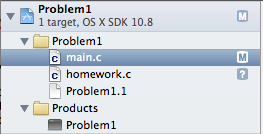
\includegraphics[width=\linewidth]{files.png}
\end{minipage} \hfill
\begin{minipage}[c]{.50\linewidth}
Normalement, une fois le projet créé, vous allez avoir 2 fichiers dans l'arborescence de votre projet: un main.c, et un nom\_du\_projet.1. Vous ne vous occupez pas du *.1, et supprimez le main.c, pour le remplacer avec le main.c fournit par Legat (simplement glisser-lâcher). Vous ajoutez aussi le homework.c dans l'arborescence (en générale, supprimer tous les *.c qu'il y a, et mettre ceux donnés par le prof). Vous pouvez coder!
\end{minipage}


\subsection{Step 5 - Execute}
\begin{minipage}[c]{.40\linewidth}
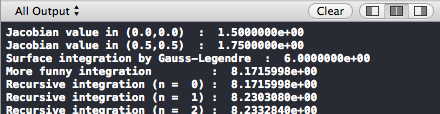
\includegraphics[width=\linewidth]{execute.png}
\end{minipage} \hfill
\begin{minipage}[c]{.50\linewidth}
Vous pensez avoir quelque chose? Vous voulez tester votre code? Rien de plus simple: appuyer sur gros bouton "Play" en haut à gauche. S'il y a des erreurs, Xcode vous le fera savoir. Sinon, vous allez pouvoir voir le résultat dans le cadre en bas à droite (comme l'image ici à gauche [les couleurs peuvent changer, vous allez plûtot avoir du texte noir sur fond blanc]).
\end{minipage}

\subsection{Step 6 - Submit}
\label{subsec:submit}
\begin{minipage}[c]{.40\linewidth}
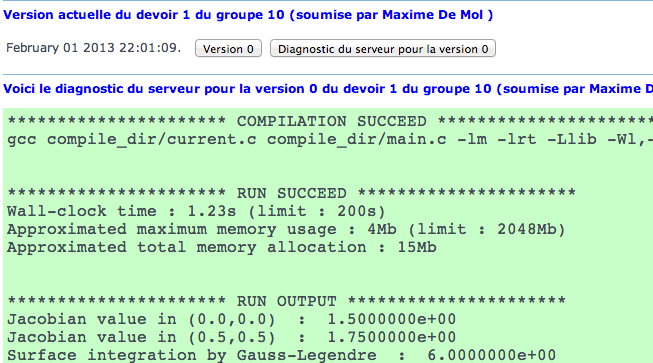
\includegraphics[width=\linewidth]{submit.png}
\end{minipage} \hfill
\begin{minipage}[c]{.50\linewidth}
Vous avez fini? Le programme semble correct? Pas d'erreurs en vue? Foncez sur le site de MECA 1120 la soumettre. Vous devez retrouver dans votre dossier projet le fichier homework.c et l'envoyer au serveur! Le diagnostic serveur est bon? Bueno! Vous avez fini!
\end{minipage}

\section{The hard way: Terminal}

Vous trouvez que Xcode, c'est trop simple? Vous voulez quelque chose de plus rapide et léger? Vous voulez programmer comme des vrais bonhommes? Alors le Terminal est pour vous!\\

\begin{lstlisting}[style=Bash]
Maxime-MBP:~ maximedemol$ echo "Welcome to the Matrix"
Welcome in the Matrix
\end{lstlisting}
\vspace{12pt}

L'inconvénient du Terminal, c'est que vous êtes moins guidé que dans Xcode. Par contre l'exécution dans le terminal est plus légère, il y a moins de chipotage, est vous pouvez vous concentrer plus sur le code lui même. Vous allez par contre avoir besoin d'un bon éditeur de texte pour éditer vos codes. Personnellement j'utilise Xcode à cet effet, mais TextMate\footnote{\url{https://github.com/textmate/textmate}} est aussi très bien côté pour ça!\\


\subsection{Step 1 - The Terminal}
\begin{minipage}[c]{.20\linewidth}

\includegraphics[width=\linewidth]{terminal.png}
\end{minipage} \hfill
\begin{minipage}[c]{.74\linewidth}
Vous pouvez trouver le terminal dans vos applications >> utilitaires! Suffit de lancer et bingo!
\end{minipage}

\subsection{Step 2 - GCC}

GCC c'est quoi? C'est le compilateur C ( et C++). C'est ce module du terminal qui va vous permettre, très bientôt de compiler vos programmes C en exécutable. Mais il y a des chances que celui-ci ne se trouve pas sur votre mac d'origine. Il faut l'installer! Pour cela, foncez à l'adresse \url{https://developer.apple.com/downloads/index.action}, inscrivez vous si c'est pas fait, et télechargez le dernier pack "Command Line Tools". Une fois installez, vous serez capable d'utiliser gcc!

\begin{lstlisting}[style=Bash]
Maxime-MBP:Desktop maximedemol$ ls
hello.c
Maxime-MBP:Desktop maximedemol$ gcc -o hello hello.c
Maxime-MBP:Desktop maximedemol$ ls
hello	hello.c
Maxime-MBP:Desktop maximedemol$ ./hello
Hello, world
Maxime-MBP:Desktop maximedemol$ 
\end{lstlisting}
\vspace{12pt}


\subsection{Step 3 - Naviguer}

Maintenant, avant de pouvoir travailler, vous devez d'abord atteindre vos fichiers! Supposons que vous avez extrait les fichiers fournis par Legat sur votre bureau. Pour y arriver, vous allez utilisez 2 commandes.

\begin{lstlisting}[style=Bash]
Maxime-MBP:~ maximedemol$ echo 'ls: voir tous les dossiers'
ls: voir tous les dossiers
Maxime-MBP:~ maximedemol$ echo 'cd: naviguer vers'
cd: naviguer vers
Maxime-MBP:~ maximedemol$ ls
Applications Desktop Documents Downloads Library Mail Movies Music
Maxime-MBP:~ maximedemol$ cd Desktop
Maxime-MBP:Desktop maximedemol$ ls
Makefile	homework.c	main.c
Maxime-MBP:Desktop maximedemol$ echo 'Nous y voila'
Nous y voila
Maxime-MBP:Desktop maximedemol$ 
\end{lstlisting}
\vspace{12pt}

\subsection{Step 4 - Editer vos fichiers}

\begin{minipage}[c]{.40\linewidth}
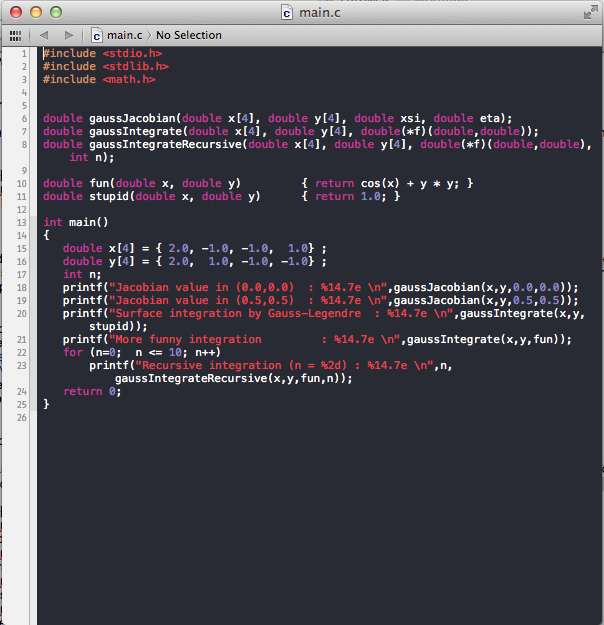
\includegraphics[width=\linewidth]{edit.png}
\end{minipage} \hfill
\begin{minipage}[c]{.50\linewidth}
Maintenant il vous faut écrire votre programme dans le fichier homework.c. Pour cela il suffit de double cliquer sur le fichier homework.c dans votre bureau. Si vous avez installé Xcode, il va s'ouvrir avec Xcode. Si vous avez TextMate, c'est TextMate qui prend le relai. Si vous voulez l'ouvrir avec autre chose, faites "ouvrir avec".
\end{minipage}

\subsection{Step 5 - Compiler}

Rien de plus simple! Legat fournit gentillement un makefile, utilisons le (commande make)!

\begin{lstlisting}[style=Bash]
Maxime-MBP:Desktop maximedemol$ make
gcc   -c  -O3 -Dgraphic -Wall -o homework.o homework.c
gcc   -c  -O3 -Dgraphic -Wall -o main.o main.c
gcc -o myFem -Wall -O3 -framework Cocoa -framework OpenGL -framework
Maxime-MBP:Desktop maximedemol$ ls
Makefile	homework.c	homework.o	main.c		main.o		myFem
Maxime-MBP:Desktop maximedemol$ 
\end{lstlisting}
\vspace{12pt}

Vous voilà en possession du fichier myFem qui est l'exécutable de votre programme!

\subsection{Step 6 - Executer}

Encore plus simple que compiler!

\begin{lstlisting}[style=Bash]
Maxime-MBP:Desktop maximedemol$ ./myFem
Jacobian value in (0.0,0.0)  :  1.5000000e+00 
Jacobian value in (0.5,0.5)  :  1.7500000e+00 
Surface integration by Gauss-Legendre  :  6.0000000e+00 
More funny integration         :  8.1715998e+00 
Recursive integration (n =  0) :  8.1715998e+00 
Recursive integration (n =  1) :  8.2303080e+00 
Recursive integration (n =  2) :  8.2332840e+00 
Recursive integration (n =  3) :  8.2334613e+00 
Recursive integration (n =  4) :  8.2334723e+00 
Recursive integration (n =  5) :  8.2334730e+00 
Recursive integration (n =  6) :  8.2334730e+00 
Recursive integration (n =  7) :  8.2334730e+00 
Recursive integration (n =  8) :  8.2334730e+00 
Recursive integration (n =  9) :  8.2334730e+00 
Recursive integration (n = 10) :  8.2334730e+00 
Maxime-MBP:Desktop maximedemol$ 
\end{lstlisting}
\vspace{12pt}

\subsection{Step 7 - Submit}

Ca marche? Ca marche bien? Foncez soumettre votre fichier homework.c qui se trouve sur le bureau! Pour plus d'info, voir section \ref{subsec:submit} page \pageref{subsec:submit}!

\section{Conclusion}

Avec ça, j'espère que tu es bien armé pour affronter le problème 1 d'éléments finis! Bonne merde à toi et à ton binôme, et bon codage!


\end{document}